%
%                       This is a basic LeTeX Template
%                       for the First Year PhD literature review 
\documentclass[a4paper,12pt]{article}
\usepackage{head,fullpage}     % Add local fullpage and head macros
\usepackage[pdftex]{graphicx}  % Add graphicx pachage with pdf flag (must use pdflatex)
\usepackage{datetime}
\renewcommand{\dateseparator}{-}
\parindent=0pt          %  Switch off indent of paragraphs 
\parskip=5pt            %  Put 5pt between each paragraph  
%
%                       This section generates a title page
%                       Edit only the sections indicated to put
%                       in the project title, your name, supervisor,
%                       project length in weeks and submission date
%
\begin{document}
\begin{minipage}[b]{110mm}
        {\Huge\bf School of Physics \\and Astronomy
        \vspace*{17mm}}
\end{minipage}
\hfill
\begin{minipage}[t]{40mm}               
        \makebox[40mm]{
        
\includegraphics[width=40mm]{crest}}
\end{minipage}
\par\noindent                                           % Centre Title, and name
\vspace*{2cm}
\begin{center}
        \Large\bf Proposed Project Title\\
        \Large\bf First Year Report and Literature Review
\end{center}
\vspace*{1.5cm}
\begin{center}
        \bf Patrick Sinclair\\                 % Replace with your name
        May 2018                          % Submission Date
\end{center}
\vspace*{5mm}
%
%                       Insert your abstract HERE
%                       
\begin{abstract}
        The abstract is a short concise outline of your 
        project area, {\bf of no more than 100 words}.
\end{abstract}

\vspace*{1cm}

\vspace*{3cm}
Signature:\hspace*{8cm}Date:

\vfill
{\bf Supervisor:} Dr. Rosalind Allen                % Change to suit
\newpage
%                                               Through page and setup 
%                                               fancy headings
\setcounter{page}{1}                            % Set page number to 1
\footruleheight{1pt}
\headruleheight{1pt}
\lfoot{\small School of Physics and Astronomy}
\lhead{Literature Review}
\rhead{- \thepage}
\cfoot{}
\rfoot{Date: \ddmmyyyydate \today}
%
\tableofcontents                                % Makes Table of Contents
\pagebreak

\section{Background}

% \begin{itemize}
%  \item Antibiotic resistance - its prevalence, not understood well
%  \item overview of gradients frm martin paper - then mention a source of gradients is biofilms
%  \item Biofilms - what are they (mention polymers perhaps)
%  \item section on industrial applications - ship hulls etc
% \end{itemize}

Since their discovery in the early 1900s \cite{bioref:first-antibiotics}, antibiotics have shaped modern medicine,
and indeed modern society as a whole.  Yet despite their prevalence, with over 260,000,000 courses of antibiotics prescribed 
in the USA alone each year \cite{bioref:antibiotics-usage-USA-2011}, very little is still known about the actual 
underlying pharmacodynamics.  I.e., how these chemicals actually regulate the growth and death of bacteria.  This 
lack of understanding is becoming increasingly significant with the rising emergence of antibiotic resistance.  
There were over 58,000 deaths in newborns under the age of a year in India in 2013 due to drug-resistant 
strains of bacteria \cite{bioref:india-death-stats}, with experts predicting that the number of deaths from 
antibiotic-resistant bacteria will number in the millions by 2050 \cite{bioref:future-death-stats}.

This project aims to shed further light on how the application of antibiotics causes bacterial populations
to evolve and proliferate over time.  In particular, in the cases of when the applied antibiotic concentration has
the form of a gradient.  A considerable portion of antibiotic research has been performed under ideal conditions
with constant, uniform antibiotic concentration \cite{bioref:Grasso-constant-antibtioic-concn}, however it has only 
recently been proposed that the effects of spatial heterogeneity may be a major factor in the emergence of resistance 
and the efficacy of drugs \cite{bioref:Zhang-effects-of-antibio-grad}.  While these concentration gradients can simply arise 
due to scenarios such as diffusion throughout body tissue \cite{bioref:tissue-antibio-grads}, the scenario which is most pertinent
to this project is that of antibiotic concentration throughout biofilms.

Biofilms arise when microbial organisms adhere irreversibly to a surface and then begin to secrete various polymers which further aid
in surface and inter-microbial attachment \cite{bioref:biofilm-formation} and creates a ``slimey'' surface.  These structures are 
particularly problematic as it is difficult to achieve sufficient drug penetration to adequately curtail microbial growth, which leads to an
increase in the persistence of infections \cite{biofilms:Costerton-biofilms-persistent}.

The ability to inhibit and even prevent biofilm growth and formation has not only a multitude of medical applications, but industrial as well.
In the shipping industry it's estimated that around 10\%, up to even 45\%, of all fuel consumption of large shipping vessels arises from overcoming the 
hydrodynamic drag caused by biofilm formation on ship hulls below the water level \cite{bioref:biofilm-fuel-consumption}.  This not only has
economic influences, but also major environmental implications.  When compared to other nations, the shipping industry is the 7th largest 
producer of CO$_2$ on the planet \cite{bioref:shipping-CO2-nation}.  Therefore, research into how these marine biofilms form and develop is 
incredibly important.

Recently, several physical methods of reducing marine biofouling have been developed, which range from physical coatings that inhibit microbial
attachment due to their topography \cite{bioref:non-toxic-antifouling-strat} to usage of ultraviolet radiation \cite{bioref:UV-biofilm-repellent}.
However, the most widespread technique is that of anti-microbial paints which are applied to the boat hulls and then leach various antimicrobial
compounds over time which inhibit biofouling \cite{bioref:antimicro-paint-desc}.  It is this latter method which is of relevant interest to this project
due to its analogous nature of applying antibiotics to bacterial biofilms.

This project will involve creating simulations of a range of scenarios where bacterial populations experience antibiotic gradients, and will
investigate how these populations develop over time.  Including but not limited to; the effects of bacterial evolution, differing types of growth-rate dependent
antibiotics and populations with heterogeneous species and resistance distributions.




% Outline\cite{bioref:KUMAR19989} the background of your subject area including the key initial
% References \cite{jr:ashkin} and reference\cite{ob:Costerton1318} textbooks \cite{ob:bornwolf}. 
% Also include some of the more
% readable articles in popular science journals \cite{jr:dholakia},
% and, where appropriate, standard textbooks \cite{ob:hechtoptics}.
% 
% The exact length of this section will depend on your subject area,
% but will generally not exceed a page and will be aimed at the 
% {\it general scientific reader}. 

\section{Review of Background Bibliography}

\begin{itemize}
  \item Causes of antibiotic crisis
  \item growth rate dependent antibiotics, $\beta$-lactams etc
  \item mention the differnt algorithms possible for the sims, gillespie etc - and give overview of what we used
  \item overview of biofouling, current ship hull anti-microbes
  \item difference of films and fouls
  \item surface colonisation
  \item opposite gradient directions for films and fouls
  \item how biocidal paint works, diffusion coefficients etc
  
 
\end{itemize}


The main articles used at this point in the project is \cite{bioref:PRL-drugGradients} and \cite{bioref:Greulich-growthDependentAntibiotics}




% In this section detail the main supporting references
% and articles \cite{jr:block} for your intended area of research
% and, most importantly, your critical evaluation of their
% relevance.  Also where your subject draws from multiple 
% disciplines, do not forget to include key reference from
% each discipline, even if they are relatively old \cite{jr:dammann}. 
% 
% 
% This is the main part of your review and is the part that
% will be of use to you when preparing for your thesis. Here try
% and identify as many of the key references as possible, and enter then
% into a {\tt BibTeX} file that you will use later. Remember that recording
% the page number, titles and details of these 
% key articles {\it now} will save you hours of
% searching through {\em Web-of-Knowledge} the day before your
% submit your thesis!
% 
% This part should be written in standard scientific language, 
% aimed at the {\em experts in the field}. This is the main part of your first year report, and is 
% expected to be 10 pages in length.

\section{Progress to Date}

Progress made so far in this project can be organised into several sections.  The initial few weeks of the project 
were spent replicating the results and techniques found in \cite{bioref:PRL-drugGradients}.  Discussion was had
on the subject of which algorithm would be optimal for updating the system over time.  Algorithms such as Gillespie\cite{bioref:Gillespie-algorithm} 
and $\tau$-leaping \cite{bioref:tau-leap-algorithm} were proposed, but 

\section{Proposal}

\begin{itemize}
 \item Writing paper on growth dependent stuffs
 \item begin work on more intricate continuum model - surface roughness and flow
 \item utilise data from AkzoNobel to accurately model growth
 \item visit AkzoNobel to undertake lab work and metagenomic analysis
\end{itemize}


In this section, detail, as far as you are currently able, 
your research plan for the second and third years of your PhD, 
drawing from the key references \cite{jr:block} that you have highlighted in your review section. 
Here, try and illustrate
your proposal, as in Figure~\ref{fig:prism} which is taken from the
same paper as the illustration references.
%
%                       Here is how to inserted a centered
%                       pdf file, this one is actually
%                       out of Maple, but it will work for other
%                       figures out of Xfig, Idraw and Xgraph
%
\begin{figure}[htb]     %Insert a figure as soon as possible
        \begin{center}
          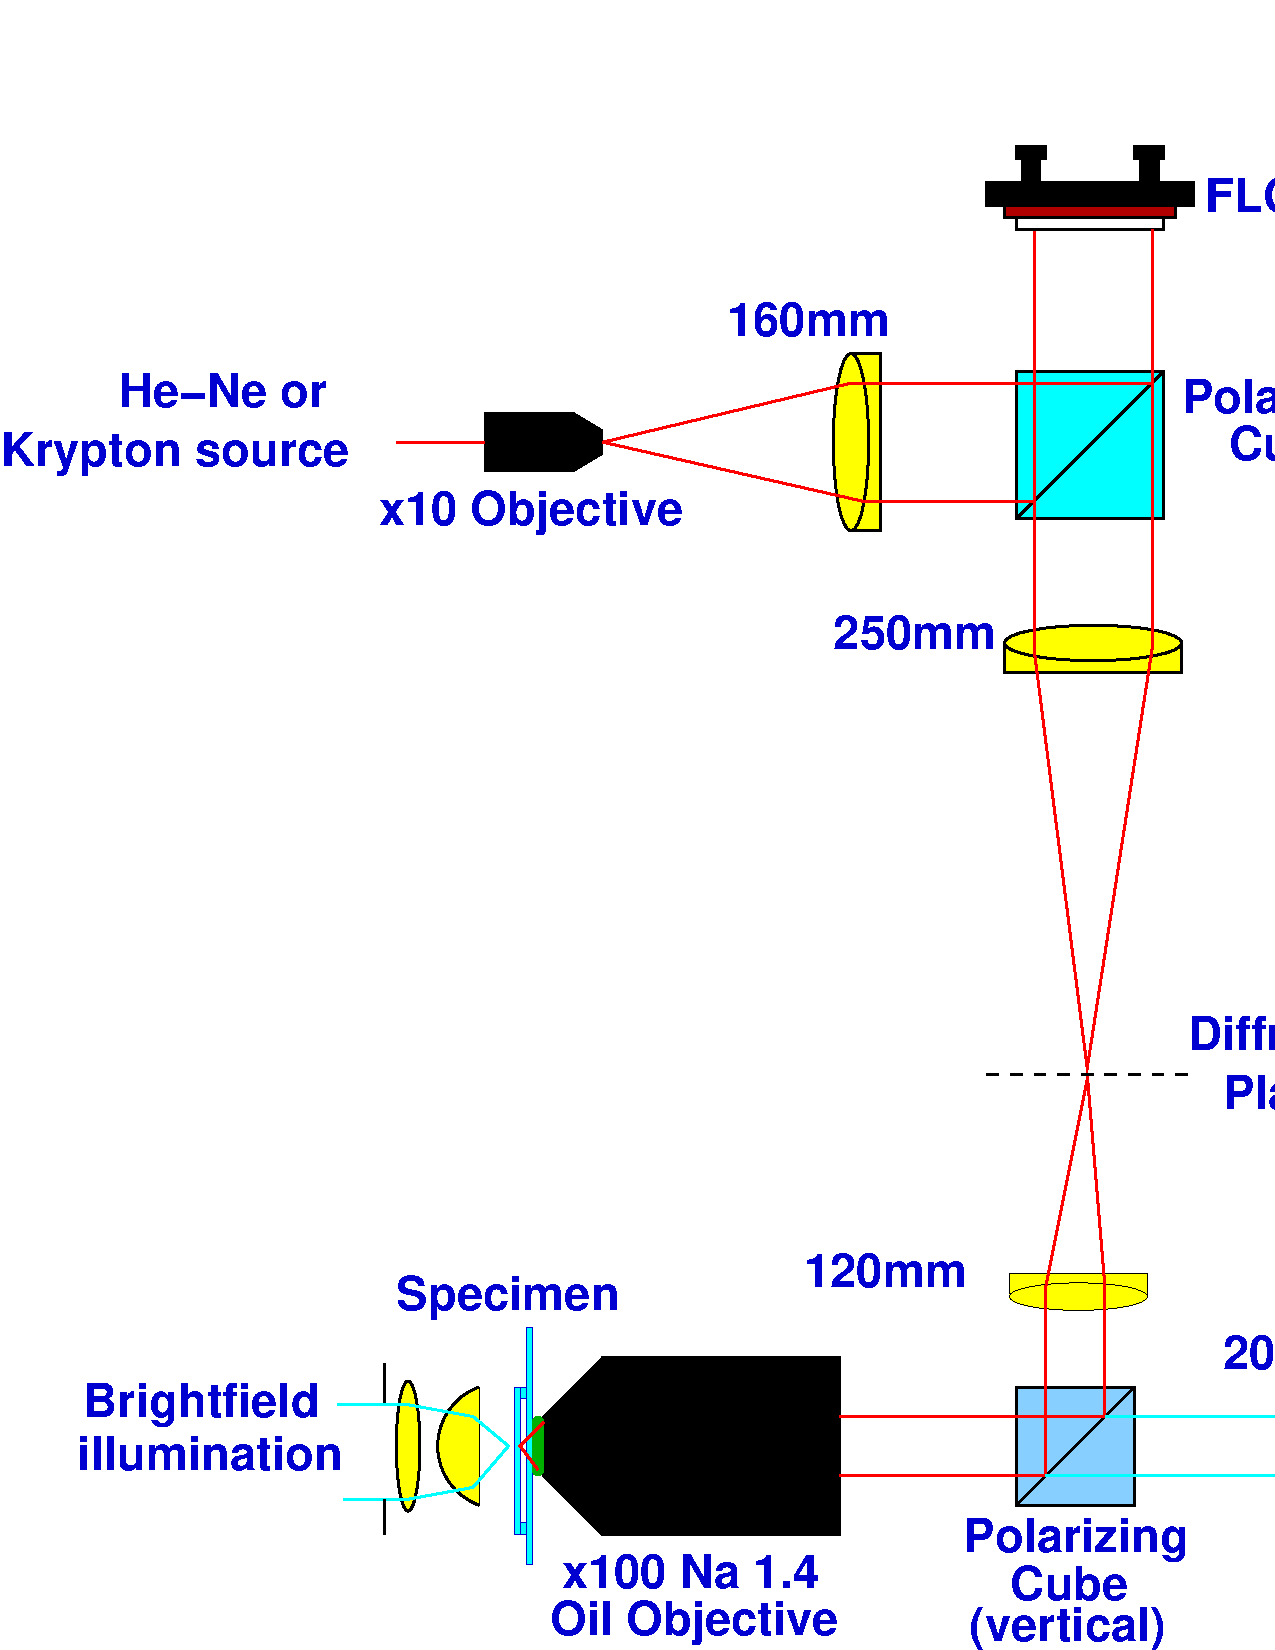
\includegraphics[width=100mm]{OpticalSystem}
\end{center}
\caption{Here is the optical system from the same paper
  as the reference drawn in {\tt xfig} and include to
  shown how such a figure in included.}
\label{fig:prism}                 % Reference label to the figure.
\end{figure}

At this stage it is {\em not} expected that this will be a fully-developed
research proposal, but is your chance to show what you have extracted from the
literature and how you see your own work will fit in. This section is
not expected to exceed 2 pages.
 
\section{Summary}

As short section highlighting the key aspect of your proposal.
At this stage this may be a bit uncertain and will be subject
to charge as the work progresses.
%            Now build the reference list
\bibliographystyle{unsrt}                      % The reference style
%                This is plain and unsorted, so in the order
%                they appear in the document.


\bibliography{BiofilmReferences}       % Multiple bib files.

\end{document}

